\todopar{Discuss the Mephisto laser head. Laser basics. Non-planar
ring oscillator. Beam shape. Frequency and intensity noise.
}
We start with a Mephisto 2 Watt laser head which has very good noise
characteristics on its own. It is a \ac{ndyag} \ac{npro} laser. It's
lasing medium is one solid piece of \ac{ndyag} with four internally reflecting
surfaces that form a ring shaped cavity. Three points define a plane, the
addition of the fourth mirror outside of this plane enables a rotation of
the polarization of the laser for each round trip around the ring. With the addition
of a permanent magnet, there will be a Faraday rotation as well which is
dependant on the direction of the laser around the ring. For one direction
the polarization rotation from the two effects are cancelled. In the other
direction, the polarization rotations are not cancelled and light leaks out
of the cavity at a rate higher than the gain of the medium due to a slight
polarization dependent reflection of the input mirror. The output beam ends
up with a very narrow linewidth but a slight elliptical shape.

Although the laser has a very good noise performance, we wish to clean it up
even further in certain regions of interest. We have assembled three systems
for this. The first is an \ac{iss} which provides active feedback to the laser
intensity. Then there is the \ac{fss} which provides active feedback to the
frequency. There is also a \ac{pmc} which is also an active feedback system. The
\ac{pmc} is used in conjunction with the \ac{iss} to ensure that we are
sensing the zero order Gaussian mode of the laser because this is what
we will ultimately be coupling into the trap cavity.

\section{Intensity Stabilization}
\todopar{Paragraph on the theory of operation}

The \ac{iss} is a genuinely eccentric animal with long, pointy ears and a fluffy
tail. It allows us to see things with incredible accuity. Far better than
previous generations of furniture.

The \ac{iss} uses a photodiode for sensing the laser power from a pick-off
beam after the \ac{pmc}. This gives us sensing of the amount of power in
the TEM00 mode of the laser we are using for our experiment. The signal is
fed back through an electronic servo to an actuator that modulates the
intensity of the beam before the \ac{pmc}. The actuator is an \ac{aom}.

\subsection{Sensing}
\todopar{Photo-electric effect, quantum efficiency}

The \ac{pd} works by the photoelectric effect. There is a quantum
efficiency associated with each \ac{pd} which is the amount of light quanta
(photons) which are converted into electrical current. This relates the
power of the incident light to the current in the output of the \ac{pd}.
We are limited by noise due to counting statistics. We want a high signal
to noise. In this case, the signal that we are concerned about is the
relative fluction in power, and so it is proportional to the DC incident
power on the \ac{pd}. The noise, as a Poissonian process, is proportional
to the square root of the DC power (or the number of photons per second).

\subsection{Feedback}
\todopar{Electronics}

The electronics were designed to reduce intensity noise above about 4 Hz to
about 1kHz or so. It is in this region where the experiment takes place.

\subsection{Actuation}
\todo{Description of Acousto-Optic Modulator}

Actuation, as mentioned above, is accomplished using an \ac{aom}. The
\ac{aom} is a device which can modulate a laser beam in both frequency
and intensity. It works by using bragg reflections in a crystal with
travelling waves. The interaction between the travelling waves and crystal
lattice divert the beam to different orders of refraction. The power in each
order is dependant on primarily the amplitude of the travelling waves. The
diffraction angle is dependant on the wavelength of the travelling waves.
We take the zero order refraction and modulate on the intensity of the
waves which, in turn, modulated the amount of power diverted into higher order
Bragg refractions.

\section{Frequency Stabilization}

\subsection{Sensing}
\subsubsection{Cavity Assembly}
\subsubsection{Cavity Suspension}
\begin{figure}[htbp]
	\centering
		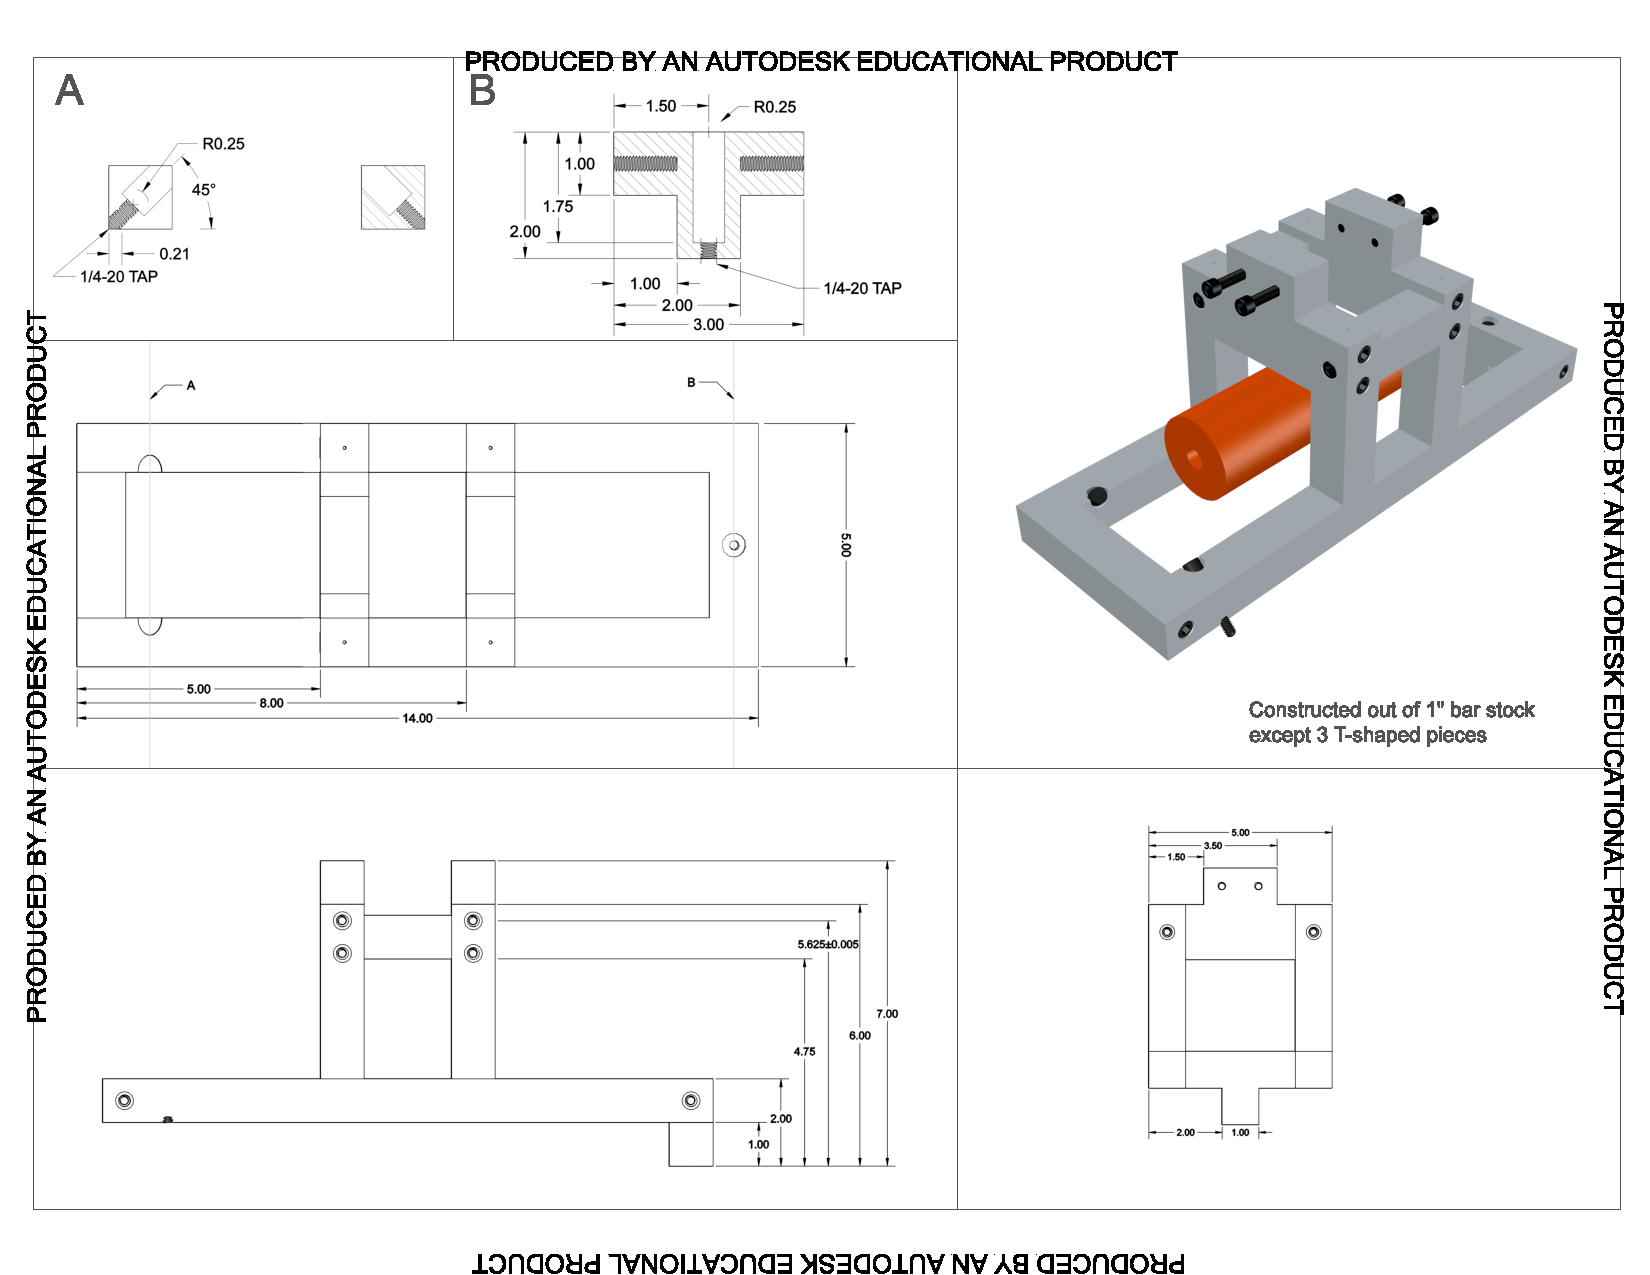
\includegraphics[width=15cm]{./figures/refcavsusdesign.pdf}
	\caption[Reference Cavity Suspension Design]{Design of the reference cavity suspension}
	\label{fig:refcav_sus}
\end{figure}

\subsubsection{PDH Locking}

\subsection{Feedback}

\subsection{Actuation}

\todopar{Add a description of the Electro-Optic Modulator}

\subsubsection{Laser Head Thermal}

\subsubsection{Laser Head Piezo-Electric Transducer}
\todopar{add description of peizo-electric effect}
\todopar{describe the effects of the piezo in-loop}

\section{Mode Cleaner}
\todopar{add description of PMC, reference Willke,98}

\subsection{Sensing}

\subsection{Feedback}

\subsection{Actuation}
